We now evaluate the potential for prediction of HS using the Traumabase. For that, we perform a prediction with CV (cf Chapter \ref{validation}) and compare it with other methods of HS evaluation. An advantage of imputation is that one can predict with various models: we compare predictions using logistic regression \cite{hosmer2013logreg}, Support Vector Machines (SVM) \cite{hearst1998SVM} and random forests \cite{svetnik2003RF} in predicting the probability of HS.

	\section{Methodology}
		\subsection{Evaluating the prediction}
The response variable in our data is binary, and we predict a probability. This, and the unbalance in the response (only 10\% of positive cases) means that the choice of metric is not straightforward. A first choice we have to make is whether we choose a threshold for the prediction (predict a positive when the predicted probability is above some value), or evaluate the predicted probability as-is.

Some metrics allow us to evaluate the predicted probability directly, such as the AUC \cite{huang2005AUC} or log-loss (minimized by the logistic regression). However, we want to be able to compare our results with those given by scores or the historical decisions of doctors, which are binary. We want to see if our predictions are able to separate patients with and without shocks at least as well as those references, so we need a metric that puts our predictions and those scores on an equal footing.

To that end, we choose a simple cost function that, given a binary prediction, assigns some user-defined cost to false negatives and false positives. That is:

$$ L(\hat{y}, y)=\frac{1}{n} \sum \limits_{i=1}^n c_1 \mathbb{1}_{y_i=1,\hat{y}_i=0} + c_2 \mathbb{1}_{y_i=0,\hat{y}_i=1}$$

To evaluate our predicted probability, we take the best value of this loss for any choice of threshold: this gives us a measure of the separation power of those predictions.

		\subsection{Choice of imputation method}
There are many methods of imputation we can choose from (cf Chapter \ref{imputation}). In order to compare them, we proceed to grouped imputation (as described in Chapter \ref{validation}) with each of them, and then perform a prediction on each imputed dataset. The resulting validation errors are presented in figure \ref{fig.imp_method}.

%\begin{figure}[h]
	\centering
   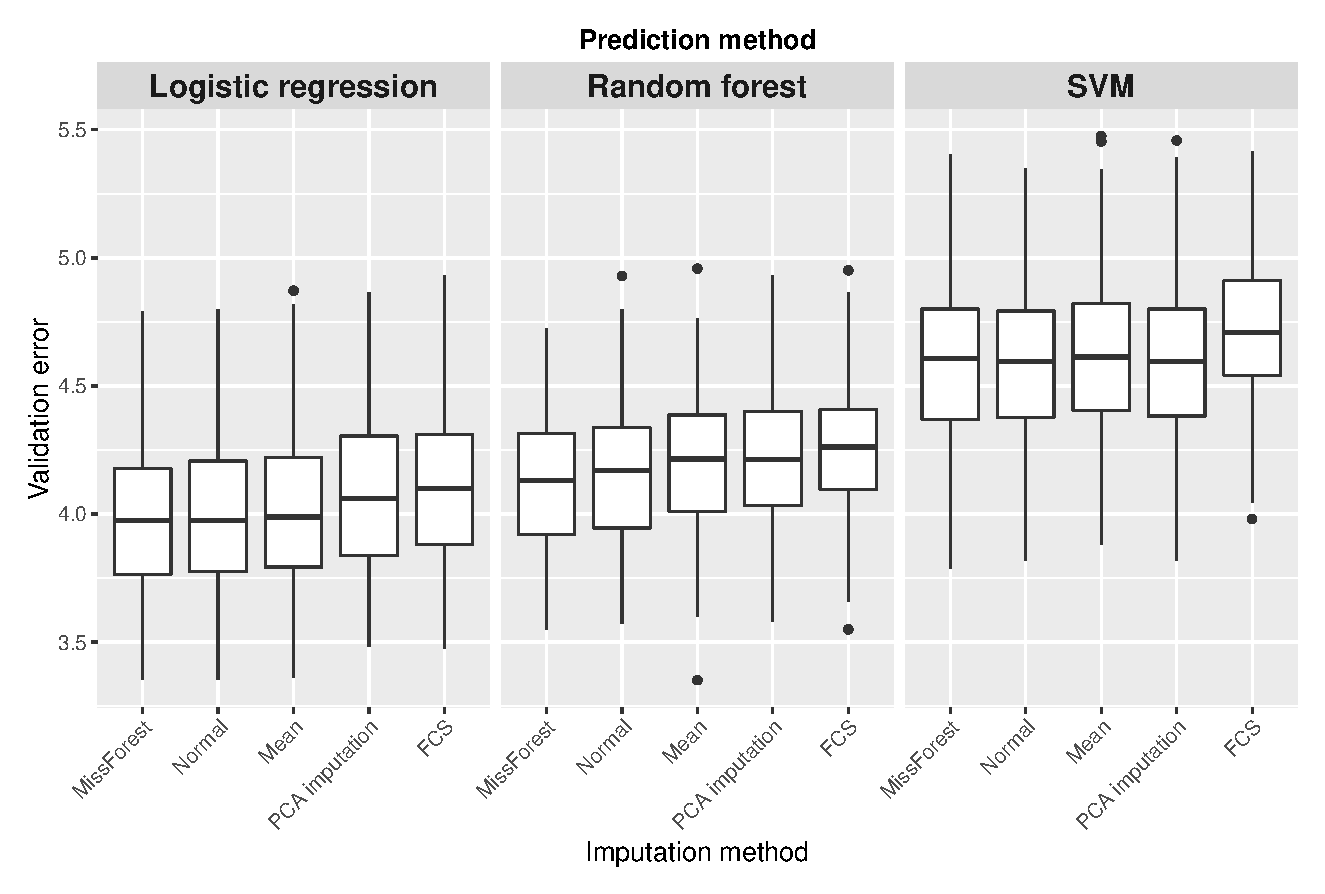
\includegraphics[scale=0.6]{Resources/imp_method}
   \caption{Prediction performance for multiple prediction and imputation methods}
   \label{fig.imp_method}
\end{figure}

It is striking that the difference between imputation methods is very small: even though there are differences in the mean performance, these differences are very small compared to the variation of the performance for different CV splits.

	\section{Results}
We performed predictions on the Traumabase data by repeatedly choosing CV splits, and then going through imputation and prediction with a logistic regression. 

In order to evaluate the prediction, we compute the loss as described above (for various choices of $c_1,c_2$) and then compare it to that obtained with the doctors' prediction (which we know because the decision to initiate the MT procedure is stored in the Traumabase), and two scores of hemorhage gravity that were designed with diagnosis in mind (as opposed to posterior analysis): the TASH (Trauma Associated Sever Hemorrhage)\cite{yucel2006tash} and ABC (Assessment of Blood Consumption)\cite{nunez2009ABC} scores.
	\label{results}